\chapter{Results So Far}

\section{Dataset}
\begin{table}[H]
\centering
\caption{Dataset funnel.}
\label{tab:funnel}
\begin{tabular}{lr}
\toprule
Stage & Objects \\
\midrule
Objaverse-LVIS objects considered & 46{,}207 \\
Passed metadata filters & 25{,}441 \\
Selected (class-agnostic) & 8{,}000 \\
Passed mesh checks & 7{,}630 \\
\textbf{Clean after preprocessing} & \textbf{7{,}467} (1{,}028 categories) \\
\bottomrule
\end{tabular}
\end{table}

\begin{table}[H]
\centering
\caption{Clean objects per group and split.}
\label{tab:groups}
\begin{tabular}{lrr@{\hspace{2em}}lr}
\toprule
Group & Objects & Categories & Split & Objects \\
\midrule
demo & 1{,}212 & 4 & train & 5{,}833 \\
related & 855 & 32 & val & 715 \\
other & 5{,}400 & 992 & test & 702 \\
 & & & test\_unseen & 217 \\
\bottomrule
\end{tabular}
\end{table}
Demo categories: chair 566, table 230, cup 208, cupboard 208. Of the 8{,}000 selected objects, 314 were flagged for having a ground plate, 56 had degenerate geometry, and 163 were flagged during preprocessing (128 hollow, 24 colourless, 11 enclosed). Preprocessing took 4.3\,h on a 4-core Kaggle CPU.

\section{Preprocessing Quality}
Figure~\ref{fig:preprocess} shows, for several objects, the coloured surface samples, the points labelled inside and the extracted watertight surface. Thin legs and the open cavity of a cup are recovered correctly. Near-surface inside ratios dropped from about 0.9 with our first voxel shell to 0.43--0.70 after switching to exact distances, which matches the expected value for a 0.4\% skin.

\begin{figure}[H]
\centering
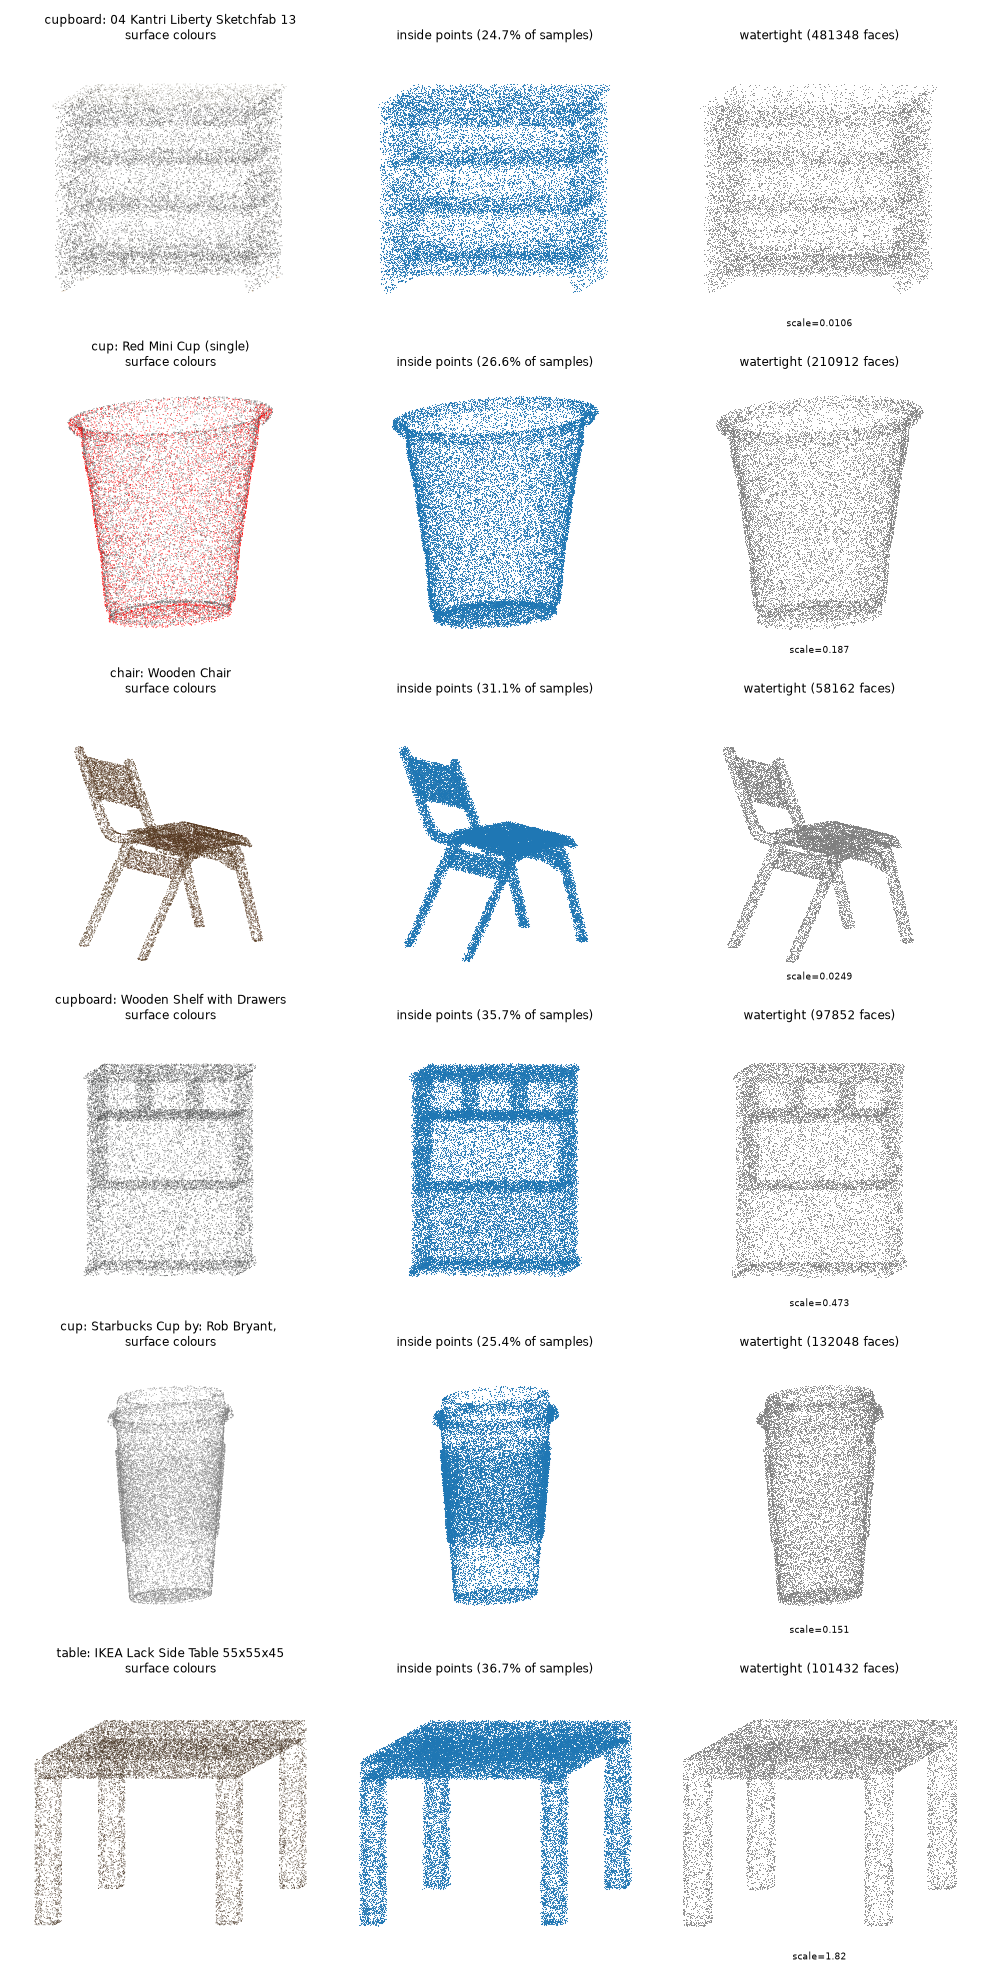
\includegraphics[width=0.75\textwidth]{preprocess_check.png}
\caption{Preprocessing output: surface colours, inside points and watertight surface.}
\label{fig:preprocess}
\end{figure}

\section{Rendering}
The first render run (16 views, 32 samples, two T4 GPUs) produced views for 3{,}118 objects in 11.95\,h at about 13.5\,s per object, covering every demo and related object. 82 objects failed and are scheduled for re-rendering. Figure~\ref{fig:renders} shows sample renders and Figure~\ref{fig:camera} the camera check.

\begin{figure}[H]
\centering
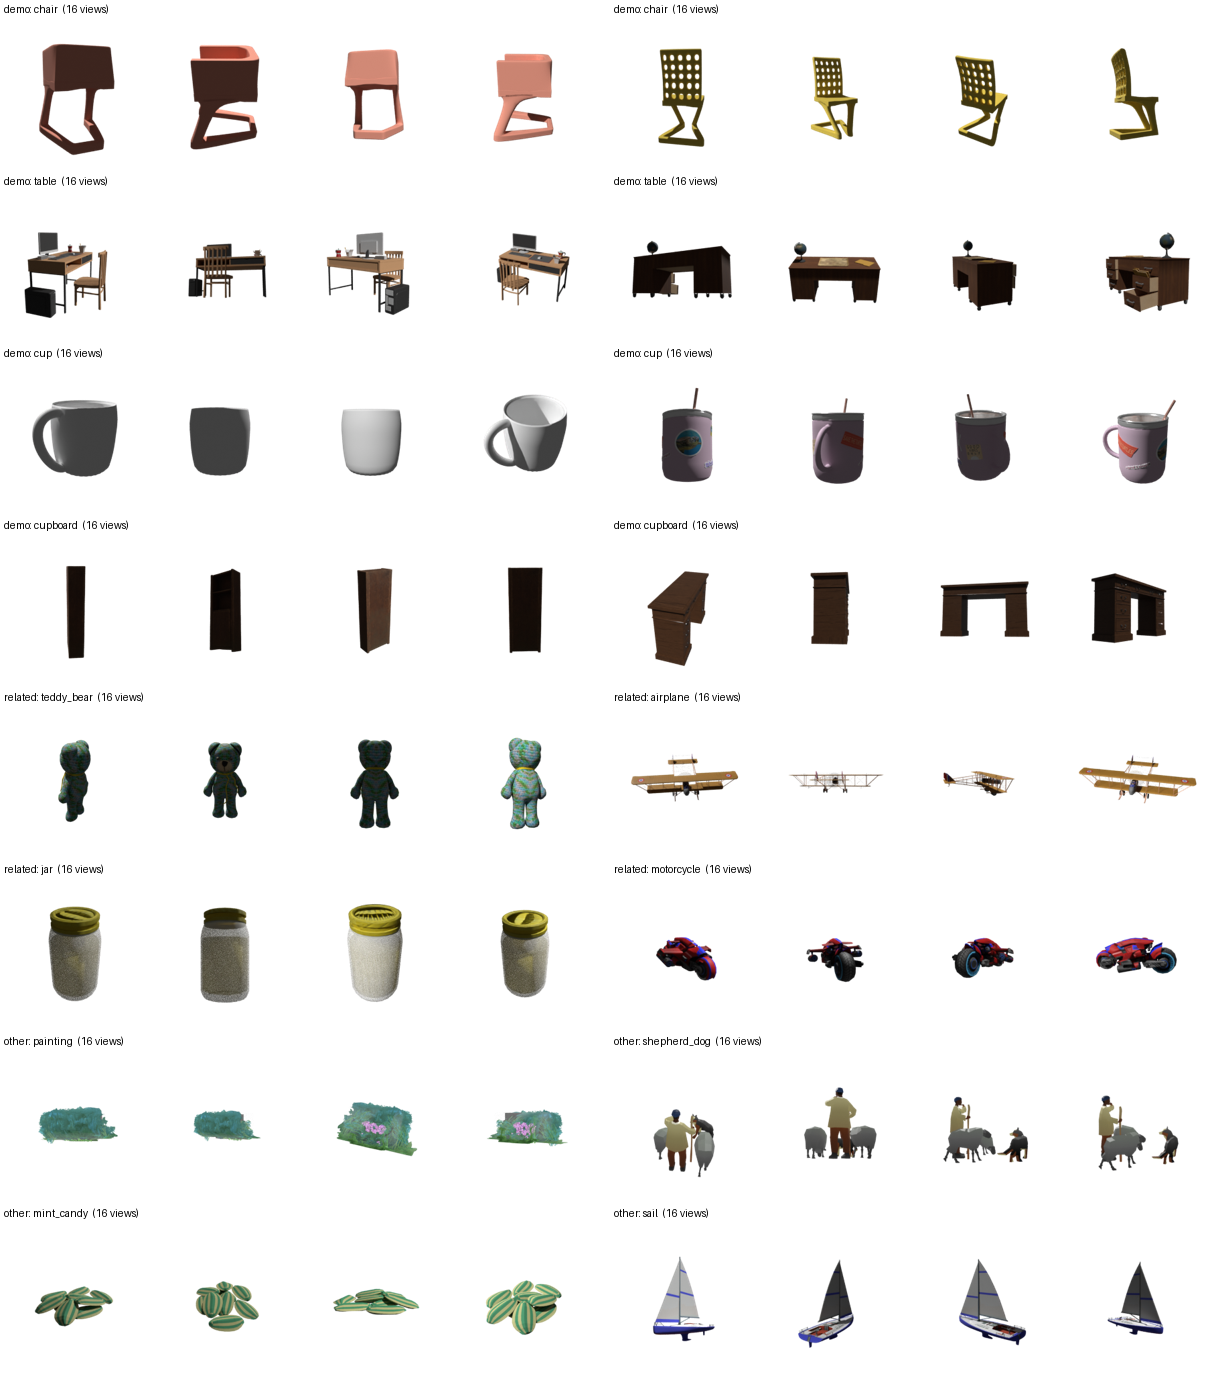
\includegraphics[width=0.85\textwidth]{kaggle_render_check.png}
\caption{Sample Kaggle renders: four of the sixteen views for objects from every group.}
\label{fig:renders}
\end{figure}

\begin{figure}[H]
\centering
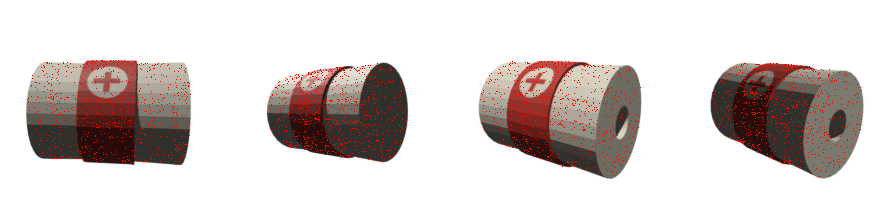
\includegraphics[width=0.85\textwidth]{camera_check.png}
\caption{Camera check: stored 3D surface points (red) projected into four rendered views.}
\label{fig:camera}
\end{figure}

\section{Generator Verification}
Before full training we checked that the generator can learn at all by training it on four objects on a CPU for 700 steps. Validation IoU rose from 0 to 0.67 and texture L1 error fell from 0.29 to 0.06. The extracted meshes have the correct position, size, orientation and colours (Figure~\ref{fig:overfit}); fine parts such as ship masts are still missing, as expected after so few steps.

\begin{figure}[H]
\centering
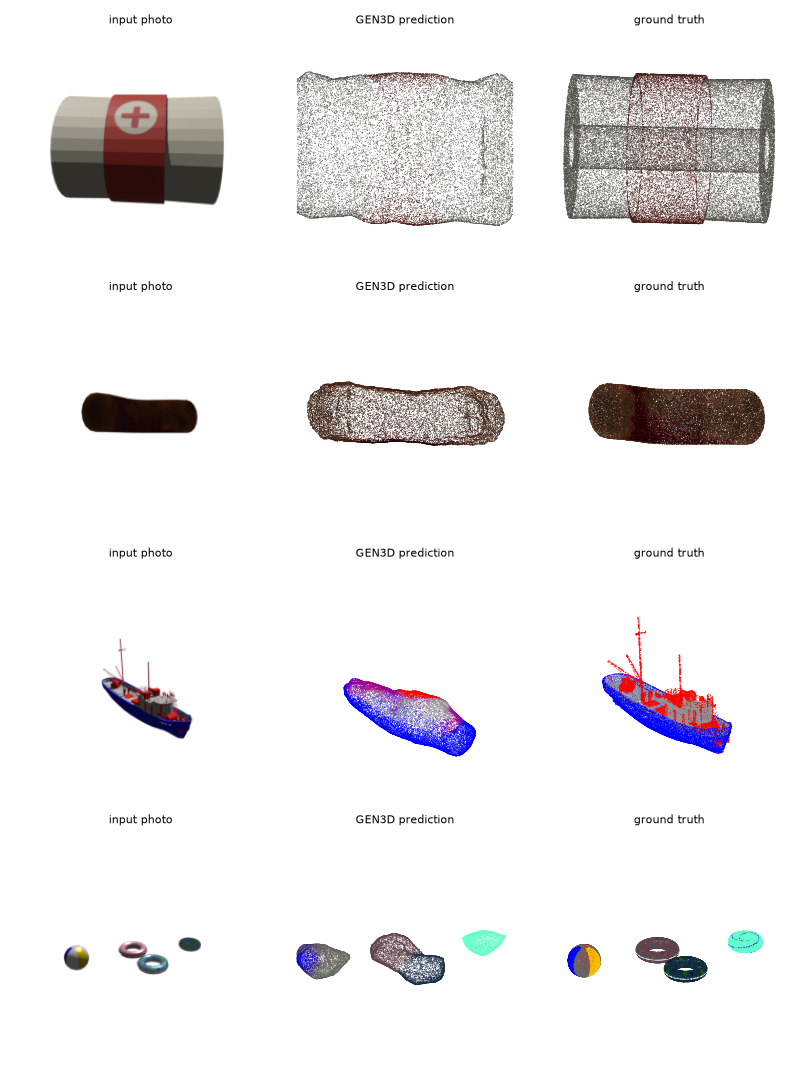
\includegraphics[width=0.7\textwidth]{overfit_check.png}
\caption{Sanity check after 700 steps on four objects: input view, GEN3D prediction and ground truth.}
\label{fig:overfit}
\end{figure}

\section{First Full Training Run (GEN3D-Gen v1)}
GEN3D-Gen v1 was trained on the train split of the 3{,}118 rendered objects (2{,}468 training and 301 validation objects) for 300 epochs on one Kaggle T4 GPU, which took 2.64 hours (about 26\,s per epoch). Validation used a fixed view per object every five epochs; the checkpoint with the best validation IoU was kept.

\begin{table}[H]
\centering
\caption{GEN3D-Gen v1 training summary. IoU is measured on the sampled query points (40\,\% of them close to the surface), so it is stricter than the volumetric IoU reported in \cite{mescheder2019onet} and not directly comparable.}
\label{tab:trainv1}
\begin{tabular}{lcc}
\toprule
 & Train (epoch 300) & Validation (best, epoch 145) \
\midrule
Occupancy IoU & 0.610 & 0.595 \
Total loss & 0.437 & 0.597 \
Colour L1 error & 0.049 & 0.089 \
\bottomrule
\end{tabular}
\end{table}

Figure~\ref{fig:trainv1} shows that the training loss falls steadily, while the validation IoU stops improving after about 35--145 epochs and the validation loss rises after epoch 150. The model starts to memorise the training objects (overfitting), which is expected with only 2{,}468 objects spread over many categories. Figure~\ref{fig:trainv1samples} shows meshes extracted from the best checkpoint: the overall size, pose and main colour are correct, and training objects such as the chair are recognisable, but thin parts (chair legs, masts) are lost and unseen objects come out as smooth blobs.

\begin{figure}[H]
\centering
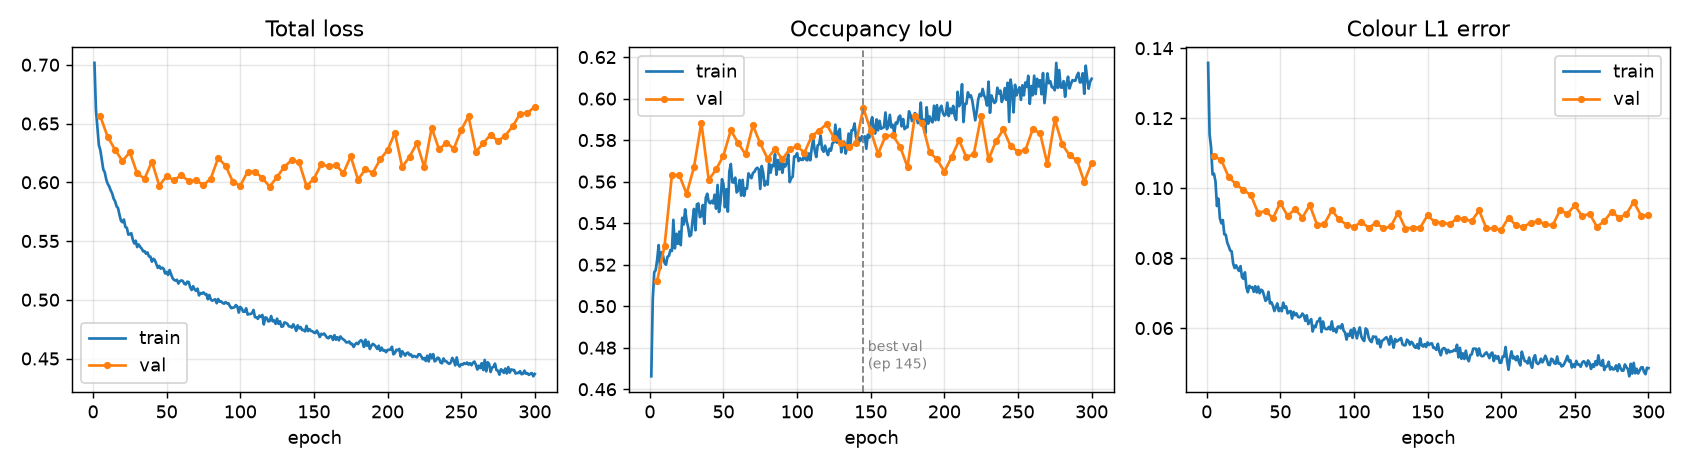
\includegraphics[width=\textwidth]{train_v1_curves.png}
\caption{GEN3D-Gen v1 training curves: total loss, occupancy IoU and colour L1 error for training and validation. The dashed line marks the best validation epoch.}
\label{fig:trainv1}
\end{figure}

\begin{figure}[H]
\centering
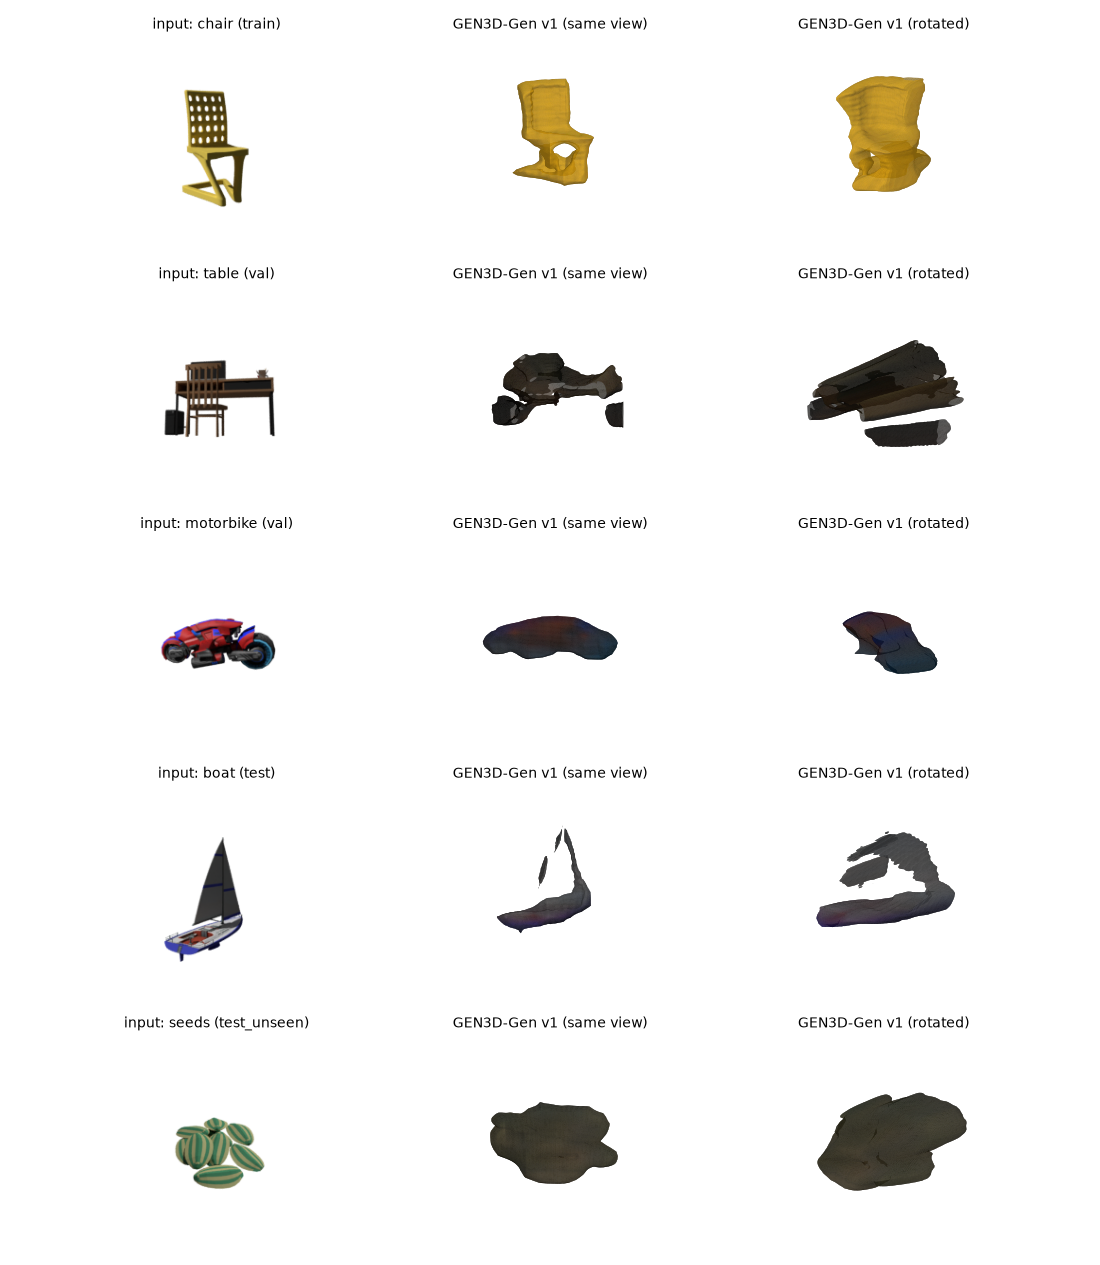
\includegraphics[width=0.85\textwidth]{train_v1_samples.png}
\caption{Meshes generated by GEN3D-Gen v1 (best checkpoint, marching cubes at $128^3$). Labels give the split of each object; only the chair was seen in training.}
\label{fig:trainv1samples}
\end{figure}

\section{Category Fine-Tuning (GEN3D-Gen v1-chair)}
To test whether more focused data helps, v1 was fine-tuned for 200 epochs (0.66\,h on a T4) on the 459 chair, stool and bench training objects, validated on the 54 chair validation objects only. Weight decay (0.05) and colour augmentation ($\pm$15\,\% brightness, contrast and saturation) were switched on. Chair validation IoU rose from 0.602 at the start of fine-tuning to 0.648 at epoch 200 and was still rising; unlike v1, the validation loss did not increase, so the regularisation stopped the overfitting. Figure~\ref{fig:v1chair} compares the two models: the chair model gives cleaner legs and a recognisable seat and back from the side on rendered chairs; on a real photo the front view improves but the depth of the chair is still wrong.

\begin{figure}[H]
\centering
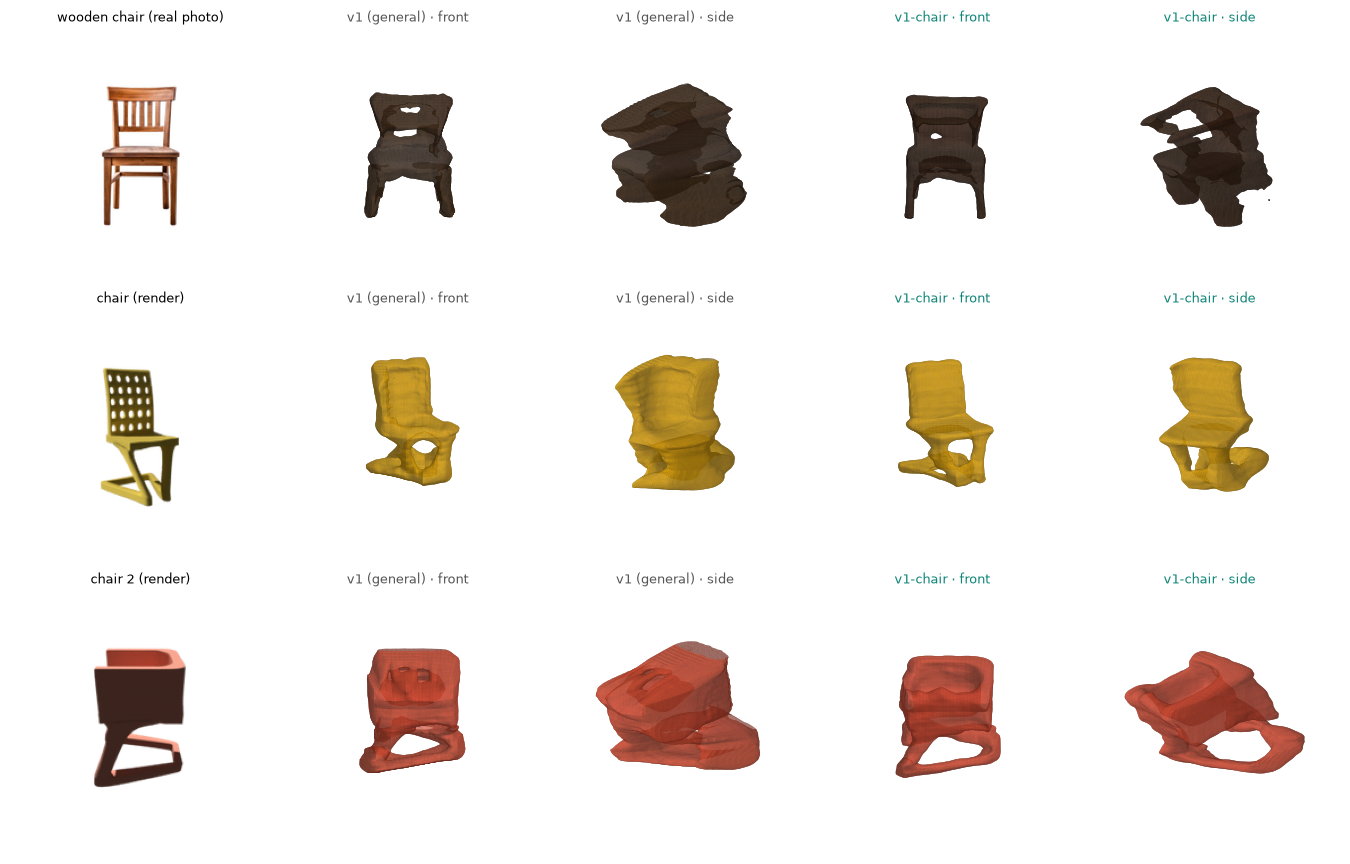
\includegraphics[width=\textwidth]{v1_vs_chair.png}
\caption{GEN3D-Gen v1 (general) vs v1-chair (fine-tuned on chairs) on one real photo and two rendered chairs, front and side views.}
\label{fig:v1chair}
\end{figure}

\section{Second Dataset and Dining-Chair Model (GEN3D-Gen v1-dining)}
Objaverse-LVIS contains only about 520 usable chairs, so we added a second dataset: Amazon Berkeley Objects (ABO)~\cite{collins2022abo}, 7{,}953 real product models with PBR textures, of which 1{,}184 are chairs. The same pipeline (download, checks, our occupancy labels, Blender renders) was extended to read ABO. To focus on one well-defined shape type for the demo, 236 dining chairs (no arms, swivel or bar chairs) were selected by product name and rendered from 24 views each; 235 passed all checks (one was rejected for exceeding 500k faces).

GEN3D-Gen v1-dining was fine-tuned from v1-chair on the 181 training dining chairs for 300 epochs (0.65\,h on a T4). Validation IoU on 27 held-out dining chairs reached 0.698 (epoch 260), with a small gap to the training IoU (0.736). Figure~\ref{fig:dining} shows the effect on a real photograph: from the side the chair now has a seat, an upright back and legs in the right places, and the colour matches the wood.

\begin{figure}[H]
\centering
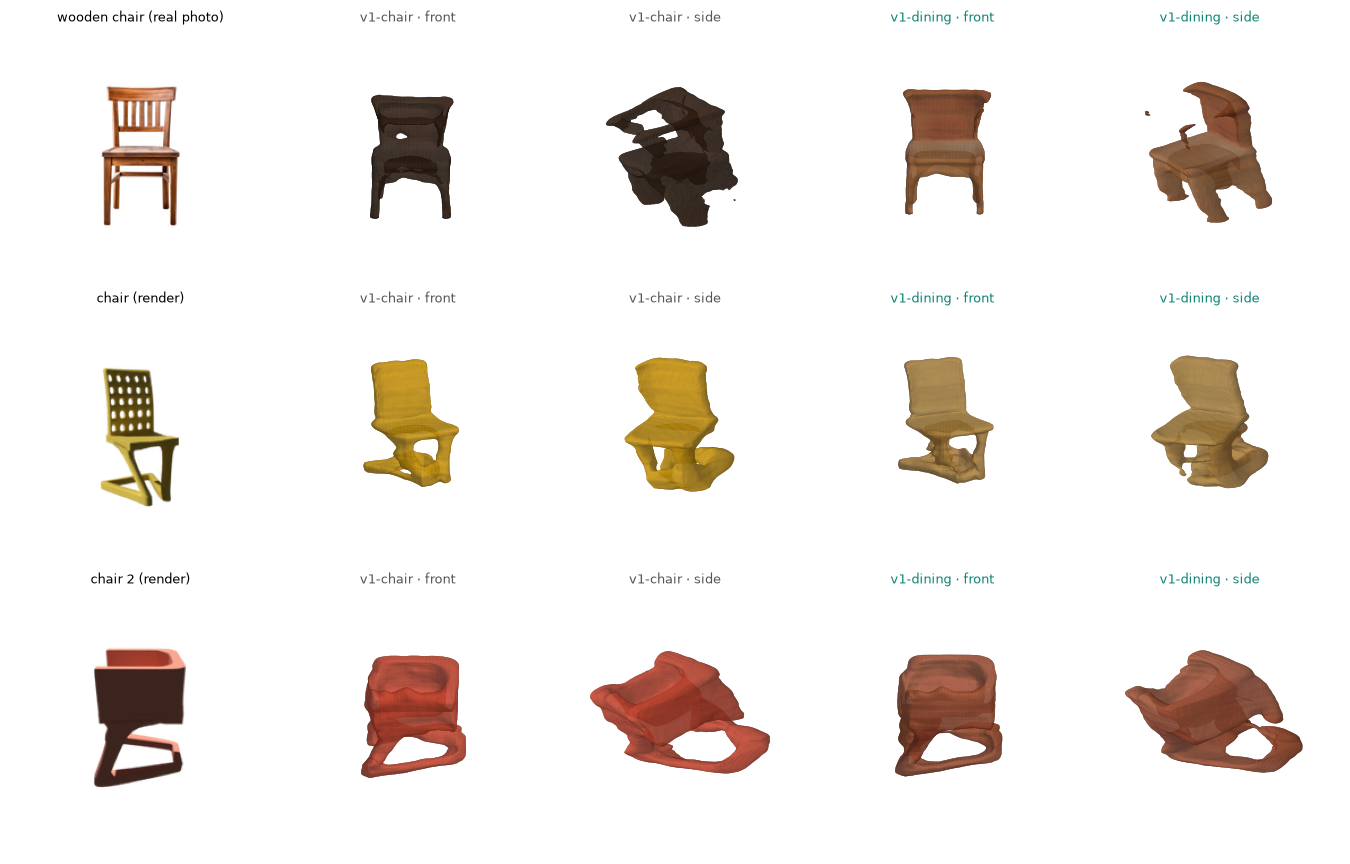
\includegraphics[width=\textwidth]{chair_vs_dining.png}
\caption{v1-chair vs v1-dining on a real photo of a wooden dining chair and two rendered chairs (front and side).}
\label{fig:dining}
\end{figure}

\section{Photo-Projected Colours}
The texture field predicts a smooth average colour, so fine detail such as slats or wood grain is lost. Because the camera of the input photo is known, every mesh vertex can be projected back into the photo. A vertex that faces the camera and is the nearest surface along its pixel (tested with a small z-buffer built from the vertices) takes the photo's pixel colour; hidden vertices keep the texture-field colour, and the two are blended at grazing angles. Figure~\ref{fig:photocol} shows the gain in realism on the visible side at no extra training cost.

\begin{figure}[H]
\centering
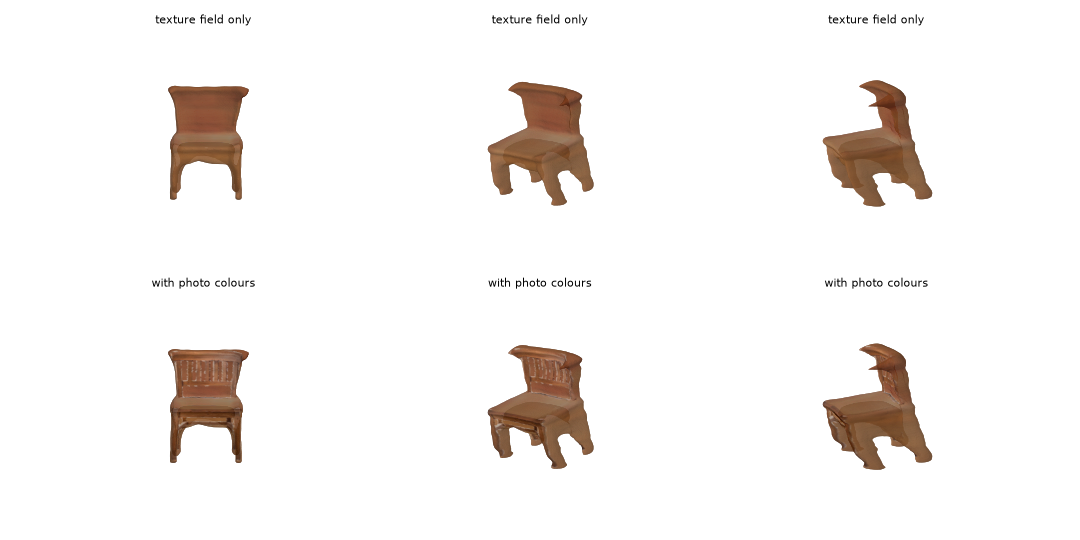
\includegraphics[width=0.9\textwidth]{photo_colours_check.png}
\caption{Same mesh, coloured by the texture field only (top) and with photo-projected colours (bottom).}
\label{fig:photocol}
\end{figure}

\section{Inside the Generator}
To understand where the errors come from, every intermediate result was visualised for one photo (Figure~\ref{fig:inside}): the DINOv2 patch features already separate the back, seat and legs; the front slice of the occupancy field is a clean chair, while the side slice shows the model hedging about the depth of the back (a faint second back on the camera side). This single-view depth ambiguity, not the recognition of the chair, is the main source of error and motivates more aligned training data.

\begin{figure}[H]
\centering
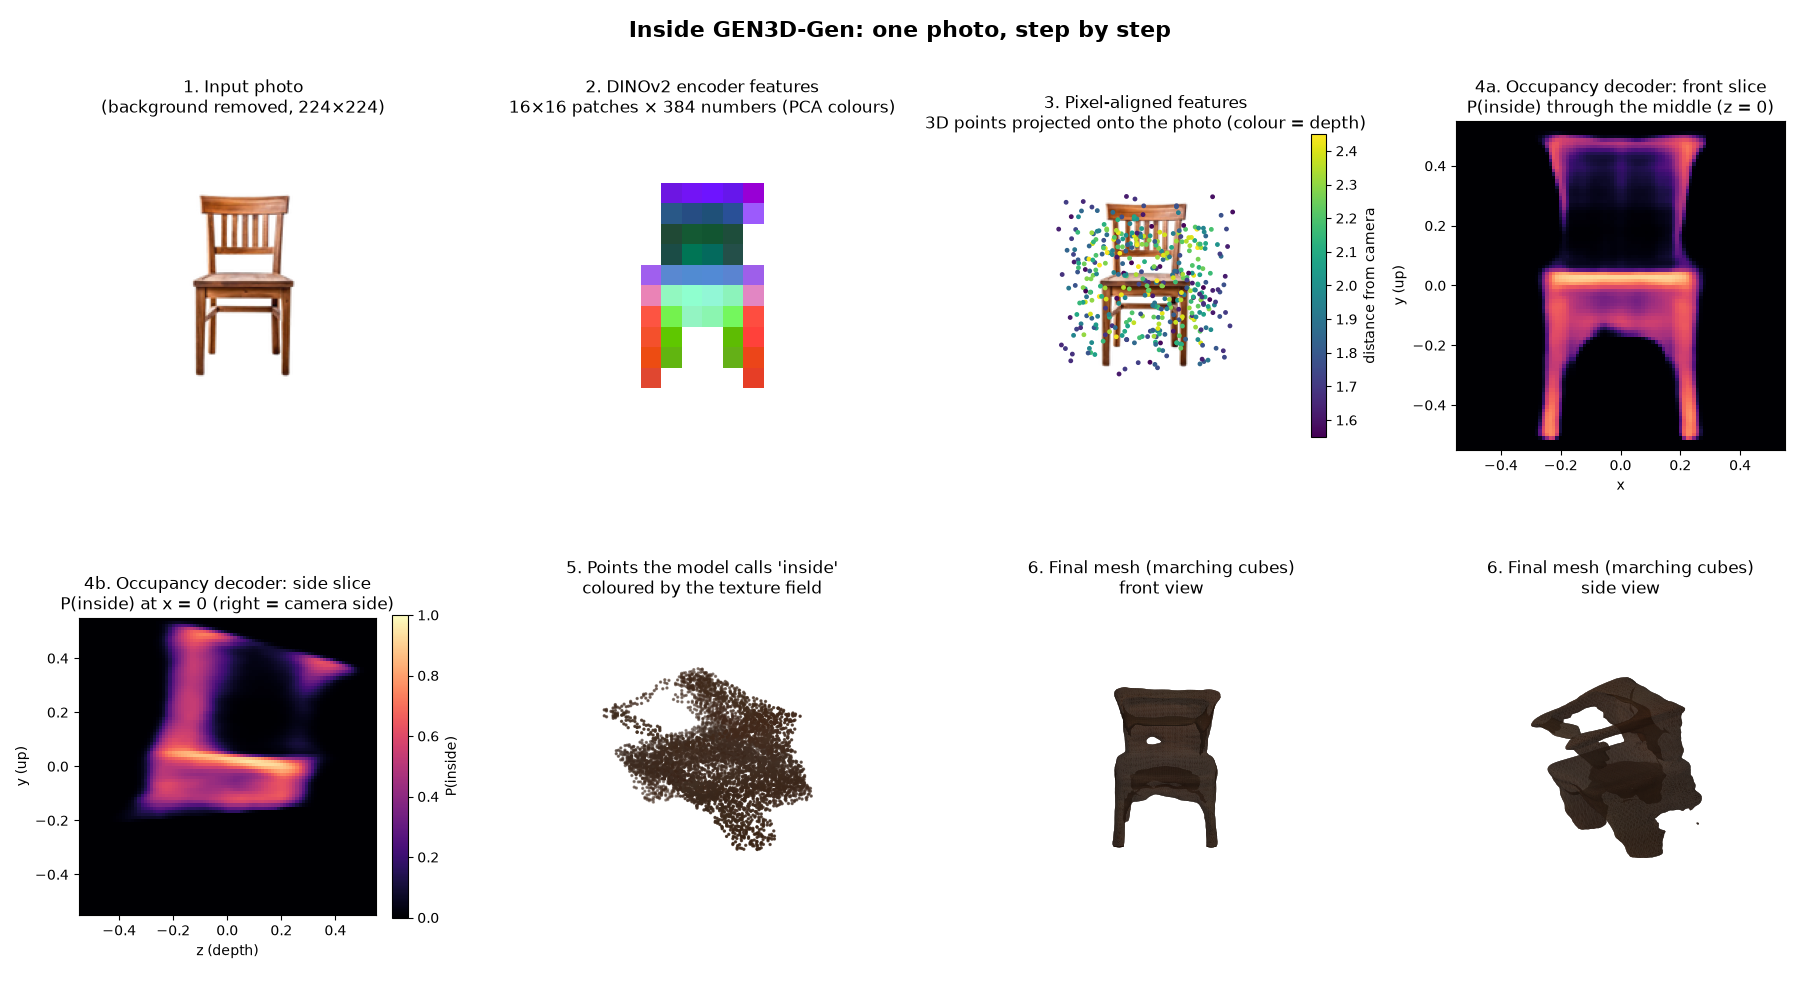
\includegraphics[width=\textwidth]{pipeline_inside.png}
\caption{Internal steps of GEN3D-Gen for one photo: input, encoder features (PCA colours), projected query points, occupancy slices (front and side), inside points with texture-field colours, final mesh.}
\label{fig:inside}
\end{figure}

\section{Following the Occupancy Networks Protocol (GEN3D-Gen v2-chair)}
To compare directly with published work we adopted the data and evaluation protocol of Occupancy Networks~\cite{mescheder2019onet}: the same ShapeNet~\cite{chang2015shapenet} chair objects (6{,}778), the same train/validation/test lists, the same 100k inside/outside points per object and the same 24 renders per object~\cite{choy2016r2n2}. Only the chair byte range (11.4\,GB) of the 73\,GB ONet archive is downloaded; a converter maps the ONet cameras into our convention (verified by projecting the point clouds onto the renders; both datasets turn out to use the same 245-pixel focal length at 224\,px). ShapeNet provides shape but no reliable colour, so this stage trains the shape only and keeps the texture field of v1-dining. Evaluation follows ONet: volumetric IoU on the uniform query points, Chamfer-L1, normal consistency, and F-score at 1\,\%. \todo{v2-chair results table vs ONet Table 1}

\section{Planned Evaluation}
\begin{itemize}[leftmargin=*]
  \item Generator: IoU, Chamfer distance and F-score@1\% on \texttt{test} and \texttt{test\_unseen}, reported per group; ablation of the encoder (DINOv2, ResNet-18 pretrained, ResNet-18 from scratch).
  \item Simplification: at 50\%, 25\% and 10\% of faces, compare PyMeshLab QEM, our QEM and D-QEM using Chamfer and Hausdorff distance (geometry), LPIPS~\cite{zhang2018lpips} and SSIM on multi-view renders (texture), and run time.
\end{itemize}
